In this section, we introduce the problem of determining every location, here defined as the center and angle of rotation, of an ellipse with fixed shape parameters, such that it contains three given points.
This problem comes up in the development of an algorithm for MCER in the next section. 
It is important to point out that no prior studies were found on it, or even on related problems.
We propose an algorithm for it that involves determining the eigenvalues of a $6\times6$ complex matrix. We also analyze its efficiency in terms of numerical accuracy and display some solutions that it was able to obtain.

\subsection{Problem definition}

Given the shape parameters of an ellipse $(a, b)$, $a > b >0$, and three points $u, v, w \in \R^2$, let $E\colon \R^2\times [0, \pi)\to\R^2$ be the coverage region of an ellipse with shape parameters $(a, b)$, we refer to the problem of obtaining $(q, \theta) \in \R^2\times [0, \pi)$, such that $\{u, v, w\} \subset \partial E(q, \theta)$ as Ellipse by Three Points Problem (E3P).
Because of its application here in our work, we are only interested in a method that can obtain every solution of E3P.

\subsection{Transforming E3P into a circle problem}

Initially, E3P is a problem with three unknown variables: $(q_x, q_y)$, and $\theta$. However, we can reduce this number to only one, as it will be shown, it is possible to obtain $q$ from $\theta$.
Let us assume that point $u$ is at the origin. If it is not, a simple translation by $-u$ applied to the three points can be made to put $u$ at the origin.
Assume as well that $(q, \theta)$ is a solution of E3P. 

Applying a rotation of $-\theta$ to the coordinate system makes the ellipse in the original solution become axis-parallel.
Then, that ellipse can be transformed into a circle of radius $b$ by squeezing the $x$-axis by $b/a$. This two-step transformation can be written as a function $\varphi\colon \R^2 \to \R^2$ defined as

\begin{equation}\label{eq:trpnts}
\varphi(p, \theta)=\left[\begin{array}{cc}
\frac{b}{a}&0\\
0&1
\end{array}\right]
\left[\begin{array}{cc}
\cos{\theta}&\sin{\theta}\\
-\sin{\theta}&\cos{\theta}
\end{array}\right]\left[\begin{array}{c}
p_x\\
p_y
\end{array}\right].
\end{equation}

An example of this transformation can be seen in \autoref{fig:circumscribed-circle}. As $\varphi^{-1}$ is well-defined, instead of solving E3P, we can work with the univariate problem of determining an angle of rotation $\theta \in [0, \pi)$ that makes the triangle with vertices $\varphi(u, \theta), \varphi(v, \theta), \varphi(w, \theta)$ be circumscribed in a circle of radius $b$. To make the notation less cluttered, we denote by $\Lambda(\theta)$ the triangle with vertices $\varphi(u, \theta), \varphi(v, \theta), \varphi(w, \theta)$.

Let $A(\theta)$ denote the area of the triangle $\Lambda(\theta)$. Using the formula given in \cite[p.~189]{johnson1960} for the radius of the circumscribed circle of a triangle, we can obtain a function $\xi \colon [0, \pi) \to \R$ given by
\begin{equation}\label{eq:circumscribed_circle_b}
\xi(\theta) = 16b^2A(\theta)^2 - \norm{\varphi(v, \theta)}^2\norm{\varphi(w, \theta)}^2\norm{\varphi(v, \theta)-\varphi(w, \theta)}^2,
\end{equation}
whose roots determine solutions of E3P.

\begin{figure}
	\centering

	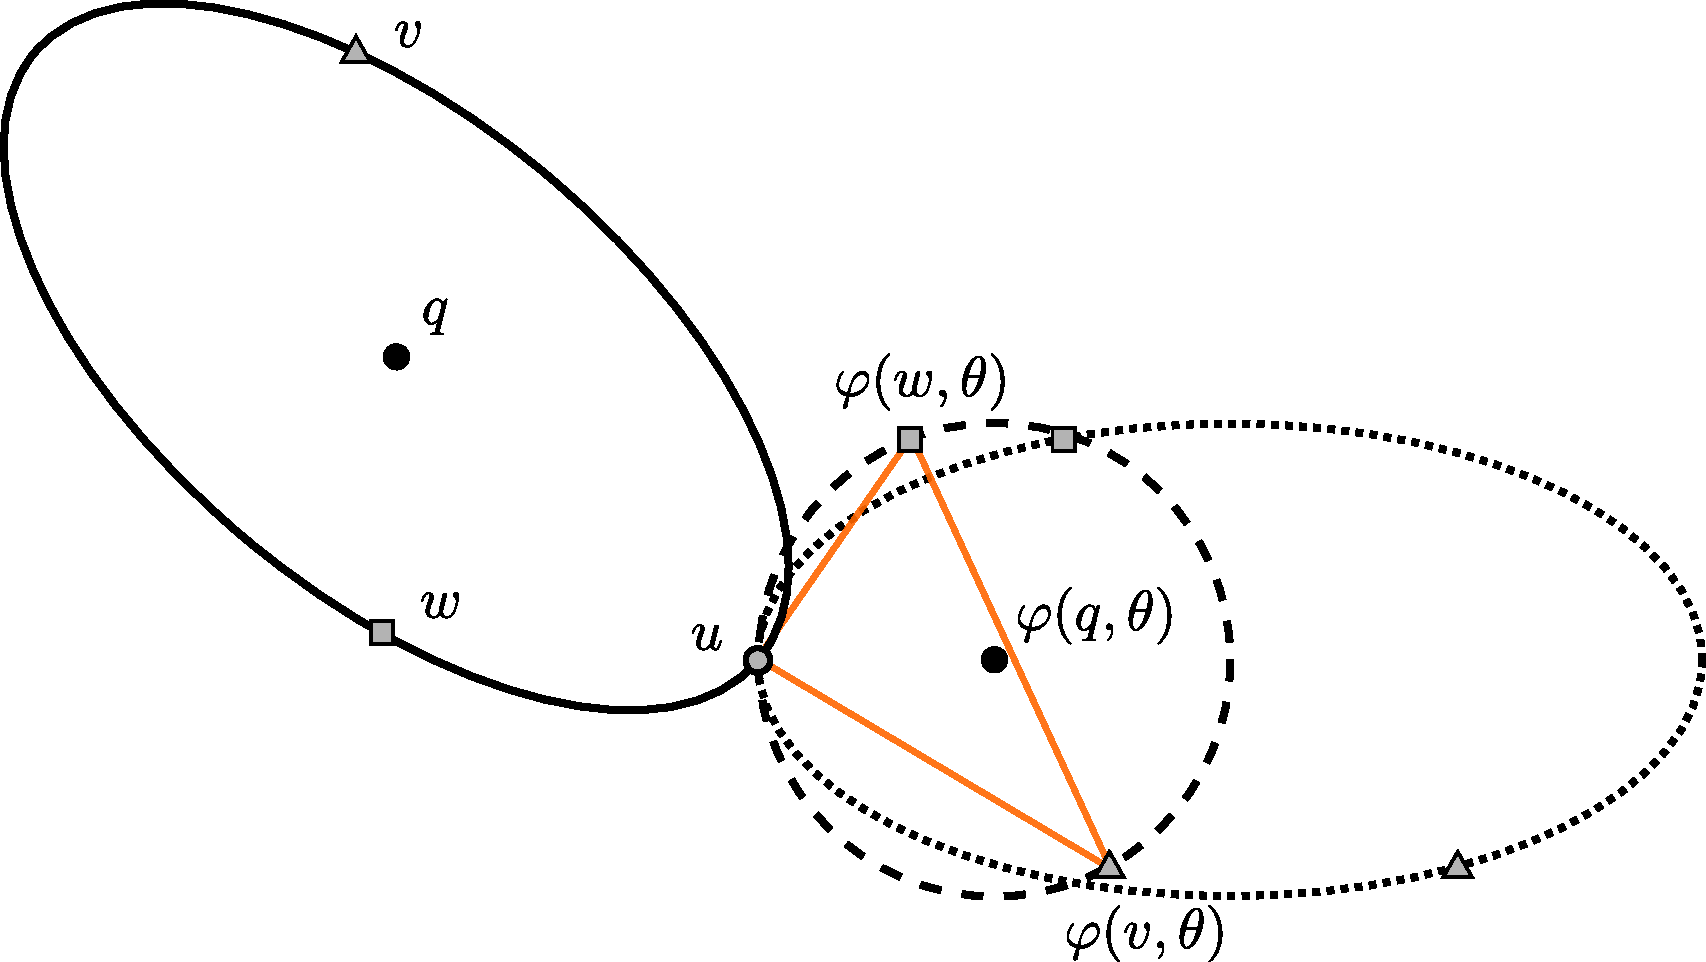
\includegraphics[scale=.3]{../tex/figures/circumscribed-circle}
	\caption{Transforming a solution of E3P into a solution of the circumradius problem.}
	\label{fig:circumscribed-circle}
\end{figure}

\begin{lem}
	E3P has at most six solutions.
\end{lem}

\begin{pf}
	The first thing to notice is that $\xi$ is a real trigonometric polynomial of degree $6$. 
	Its term of highest degree is the multiplication of the norms $\norm{\varphi(v, \theta)}^2\norm{\varphi(w, \theta)}^2\norm{\varphi(v, \theta)-\varphi(w, \theta)}^2$. In \cite[p.~150]{powell}, where a definition of real trigonometric polynomial is also given, it is stated that a $n$-degree real trigonometric polynomial can have up to $2n$ roots in $[0, 2\pi)$. Therefore, E3P has at most $12$ solutions in $[0, 2\pi]$.
	Half of these solutions, though, are duplicated as ellipses are symmetric to their axis.
\end{pf}

\subsection{Converting $\xi$ into a polynomial}

In \cite[p.~195]{horn}, a theorem is presented stating that for every univariate polynomial of degree $n$, there exists a companion matrix which is a $n\times n$ matrix, such that its eigenvalues are the zeros of that polynomial. Finding every eigenvalue of a matrix can be done using the QR algorithm, which runs in $\bigO(n^3)$ and uses $\bigO(n^2)$ memory (a very complete introduction to it can be found in \cite{watkins:2008}). Therefore, finding the roots of a univariate polynomial of degree $n$ can be done in $\bigO(n^3)$. Because of that, we use an approach published in  \cite{boyd:2006} to convert real trigonometric polynomials into complex polynomials to convert $\xi$ into a complex polynomial of degree $12$.

Replacing $\cos{\theta}$ and $\sin{\theta}$ by their identities defined as follows
\begin{align}\label{eq:complex_trig_cos}
\cos{\theta} &= \dfrac{e^{i\theta} + e^{-i\theta}}{2},\\
\label{eq:complex_trig_sin}
\sin{\theta} &= \dfrac{e^{i\theta} - e^{-i\theta}}{2i}.
\end{align}

It is possible to show that with that substitution, plus changing the variable to $z=e^{i\theta}$, we obtain the following function $g : \mathbb{S} \mapsto \mathbb{C}$, with $\mathbb{S}$ being the unit complex circle ($\mathbb{S} = \{z \in \mathbb{C} : |z|=1\}$, and $g(z) = \sum_{k=0}^{12} c_k z^{k-6}$. Multiplying $g$ by $z^6$, and extending the domain to $\mathbb{C}$, we obtain the degree-$12$ complex polynomial $h(z) = z^6g(z)$.

We can cut in half the degree of the complex polynomial by observing that $angle(-z) = \pi + angle(z)$, which implies, because of the symmetry of ellipses, that $g(z) = g(-z)$. Therefore, every odd degree coefficient of $h$ is zero. Using the substitution $y = z^2$, we obtain a degree-$6$ complex polynomial $f(y) = \sum_{k=0}^{6} c_{2k} y^{k}$. Then, from the roots of $f$ we obtain the set of solutions of E3P:
$\{(u + \varphi^{-1}(\hat{q}, angle(\hat{y})/2), angle(\hat{y})/2) \colon f(\hat{y})=0\}$.